\section{GUI-Entwürfe}
\label{sec:gui-entwuerfe}

\subsection{Sidebar}
\label{subsec:sidebar}

Die Sidebar beinhaltet von oben nach unten das Logo, einen Button zum Speichern, einen Button zu Overleaf, einen Button
zum Exportieren, eine Statusanzeige, einen Graphmodus-Toggle und einen Button zum Schließen.

\subsubsection{Export}

Nachdem der Export-Button gedrückt wurde, erscheint ein Popup-Fenster.

\begin{center}
  \begin{minipage}{0.5\linewidth}
    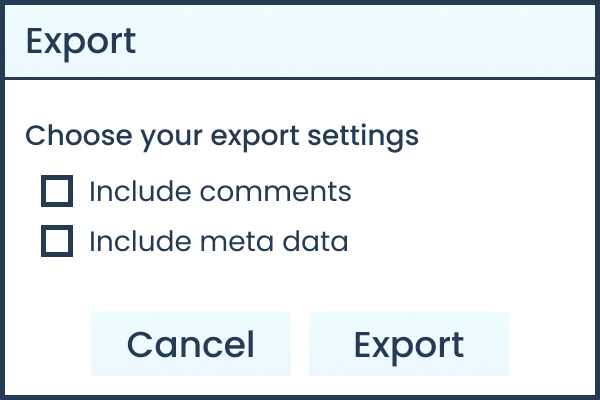
\includegraphics[width=\textwidth]{assets/img/Export_Box}
    \captionof{figure}{Export-Box mit Export"=Attributauswahl}
  \end{minipage}
\end{center}

Im Export-Fenster kann der User Exporteinstellungen wählen und den Export bestätigen oder abbrechen.

\subsubsection{Overleaf-Link}

Durch Klicken des Overleaf-Symbols gelangt man zur verknüpften Overleaf-Projektseite.

\subsubsection{Graphmodus-Toggle}

Der Button wechselt zwischen dem Graphmodus und dem Standardmodus.

\subsection{Arbeitsbereich}
\label{subsec:arbeitsbereich}

Der Arbeitsbereich, also der Bereich, der nicht Sidebar ist, besitzt drei verschiedene Modi.

\subsubsection{Standardmodus}

\begin{minipage}{\linewidth}
  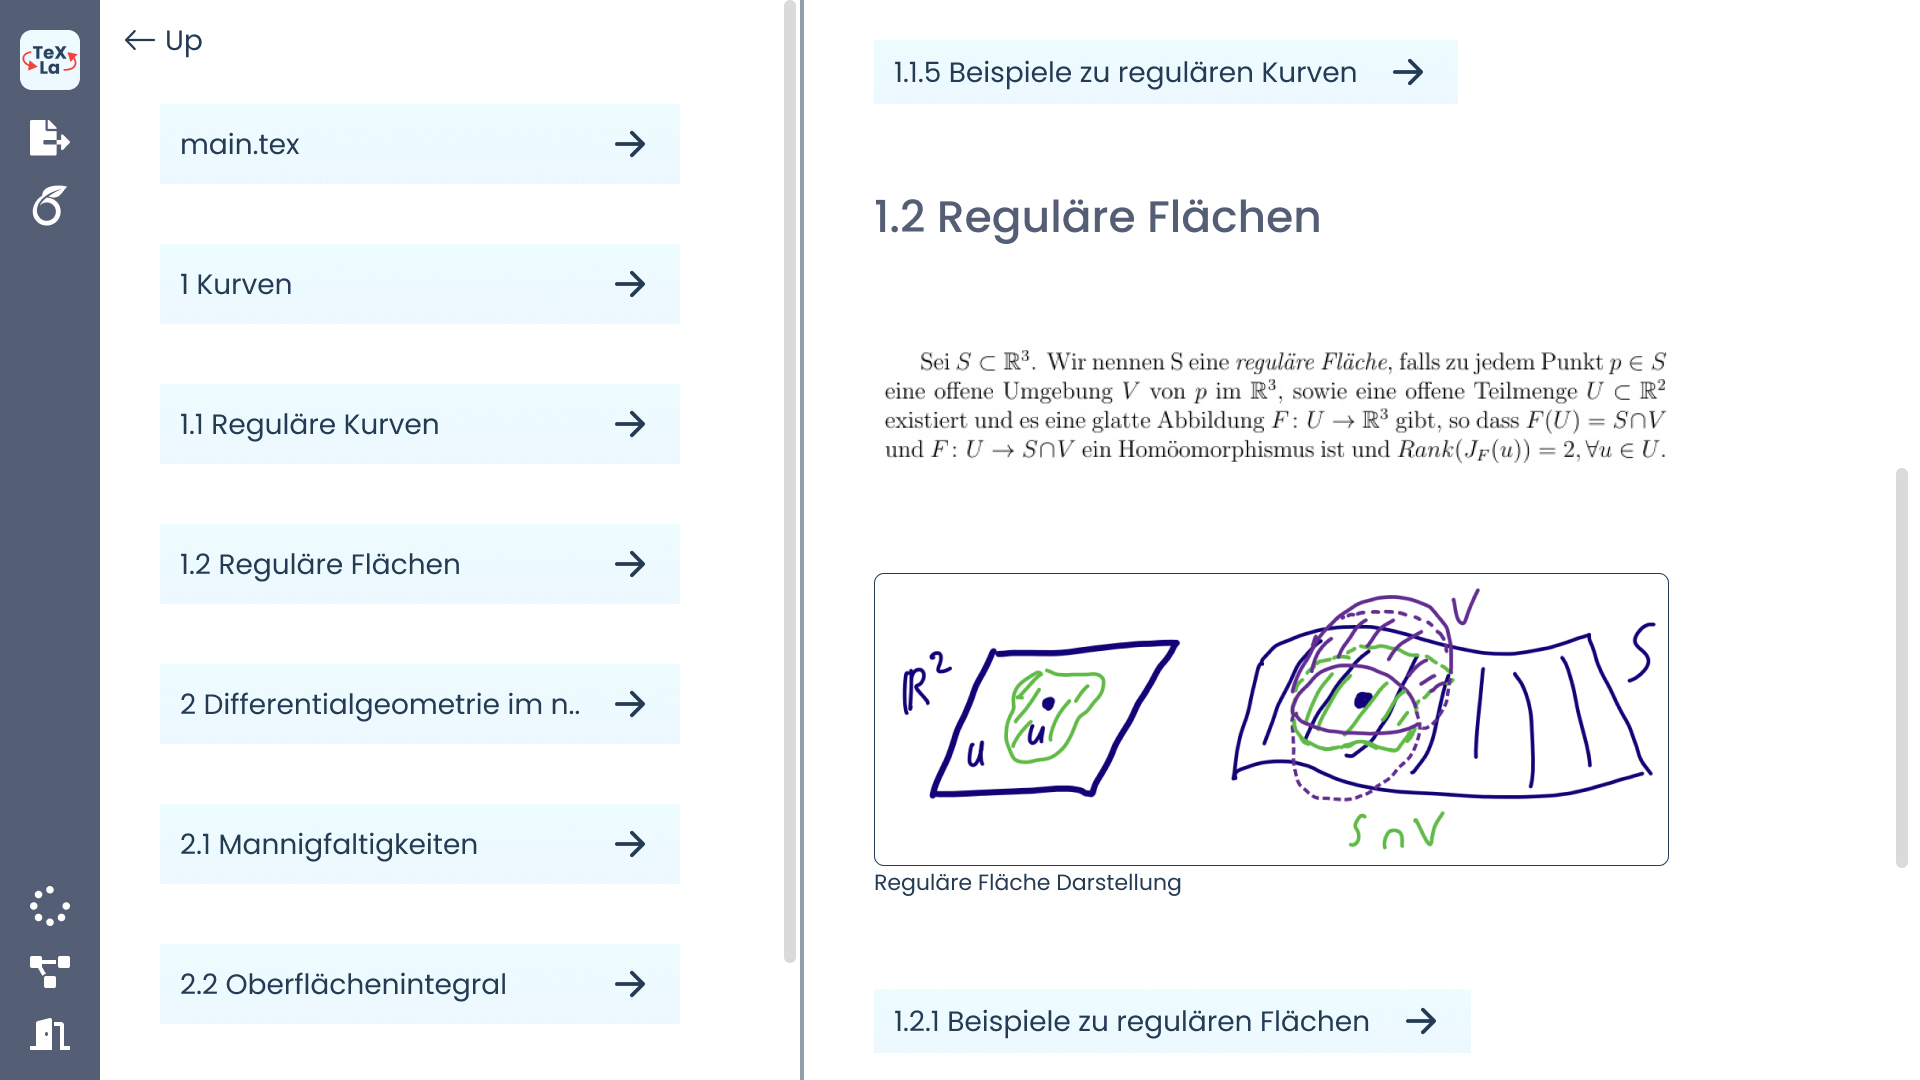
\includegraphics[width=\textwidth]{assets/img/Standardansicht}
  \captionof{figure}{Standardmodus}
\end{minipage}

In diesem Modus stehen die meisten Funktionen von \texla{} zur Verfügung.

Die rechte Spalte beinhaltet alle Strukturelemente bis Ebene $i$.
Dabei werden Expandables der Ebene $i$ in Kompaktform dargestellt und alle anderen Elemente in vollständiger Form.
In der linken Spalte werden alle Expandables des Dokuments bis zur Ebene $i-1$ in ihren Kompaktformen in
Reihenfolge des Vorkommens im Dokument dargestellt.

Auf beiden Seiten kann gescrollt werden, um den gesamten Inhalt einzusehen.
Ein Klick auf eine Kompaktform auf der linken Seite führt zu einem Sprung an die jeweilige Stelle auf der rechten Seite.

\subsubsection{Bearbeitungsmodus}

\begin{minipage}{\linewidth}
  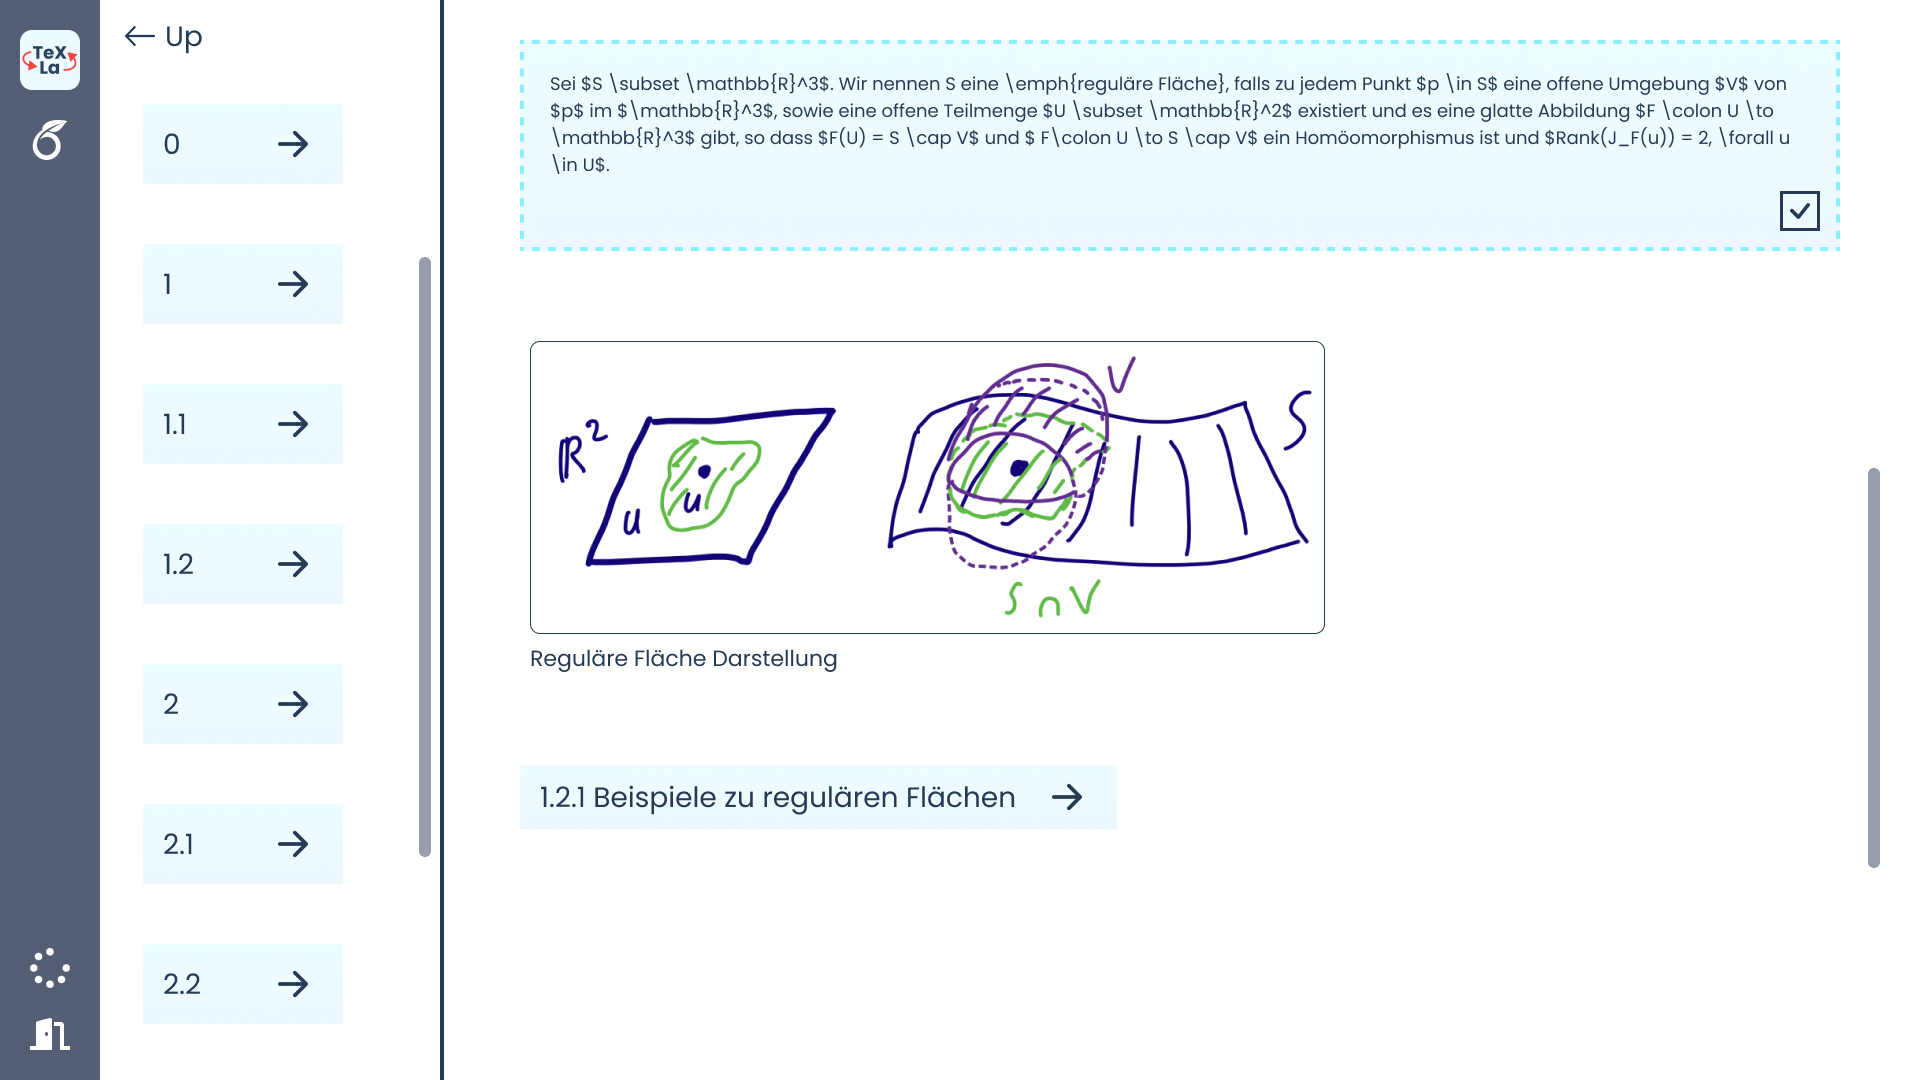
\includegraphics[width=\textwidth]{assets/img/Editor_View}
  \captionof{figure}{Bearbeitungsmodus}
\end{minipage}

Beim Bearbeiten eines Elements wechselt der Navigationsbereich in den Bearbeitungsmodus.
Hier wird die linke Spalte nur noch komprimiert dargestellt und die rechte Spalte vergrößert sich.
Das zu bearbeitende Element wird im Minieditor in Quelltext angezeigt.
Der User kann die nötigen Bearbeitungsschritte tätigen.
Durch Klicken des Bestätigen-Buttons werden die Änderungen übernommen, der User verlässt den Bearbeitungsmodus und
gelangt in den Standardmodus zurück.

\subsubsection{Graphmodus}

\begin{minipage}{\linewidth}
  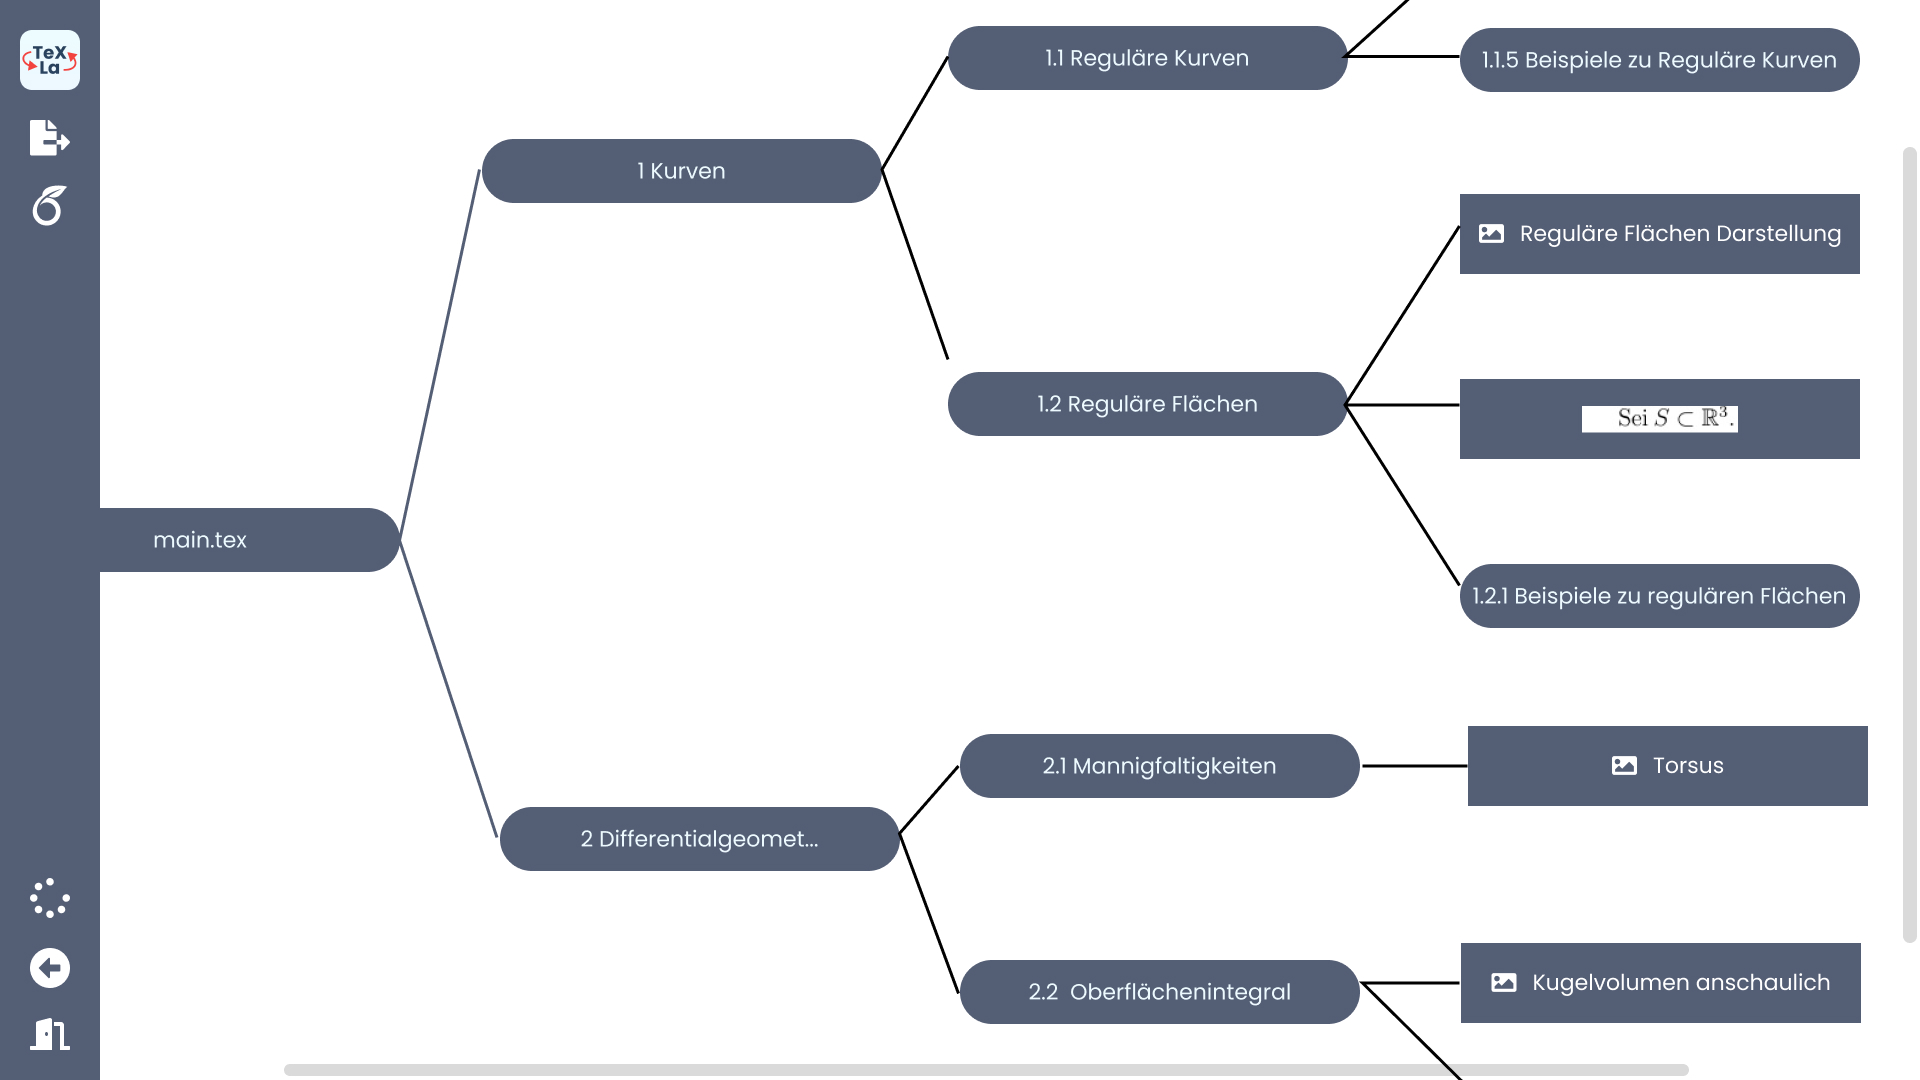
\includegraphics[width=\textwidth]{assets/img/Graphansicht}
  \captionof{figure}{Graphmodus}
\end{minipage}

Im Graphmodus wird das Dokument als Graph dargestellt.
In diesem Modus erhält der User Überblick über das Dokument und er kann die Elemente des Dokuments ebenenübergreifend
restrukturieren.
Im Graphmodus navigiert man durch Scrollen.

\subsection{Interaktion mit Elementen}
\label{subsec:interaktion-mit-elementen}

\subsubsection{Element fokussieren}

\begin{minipage}{\linewidth}
  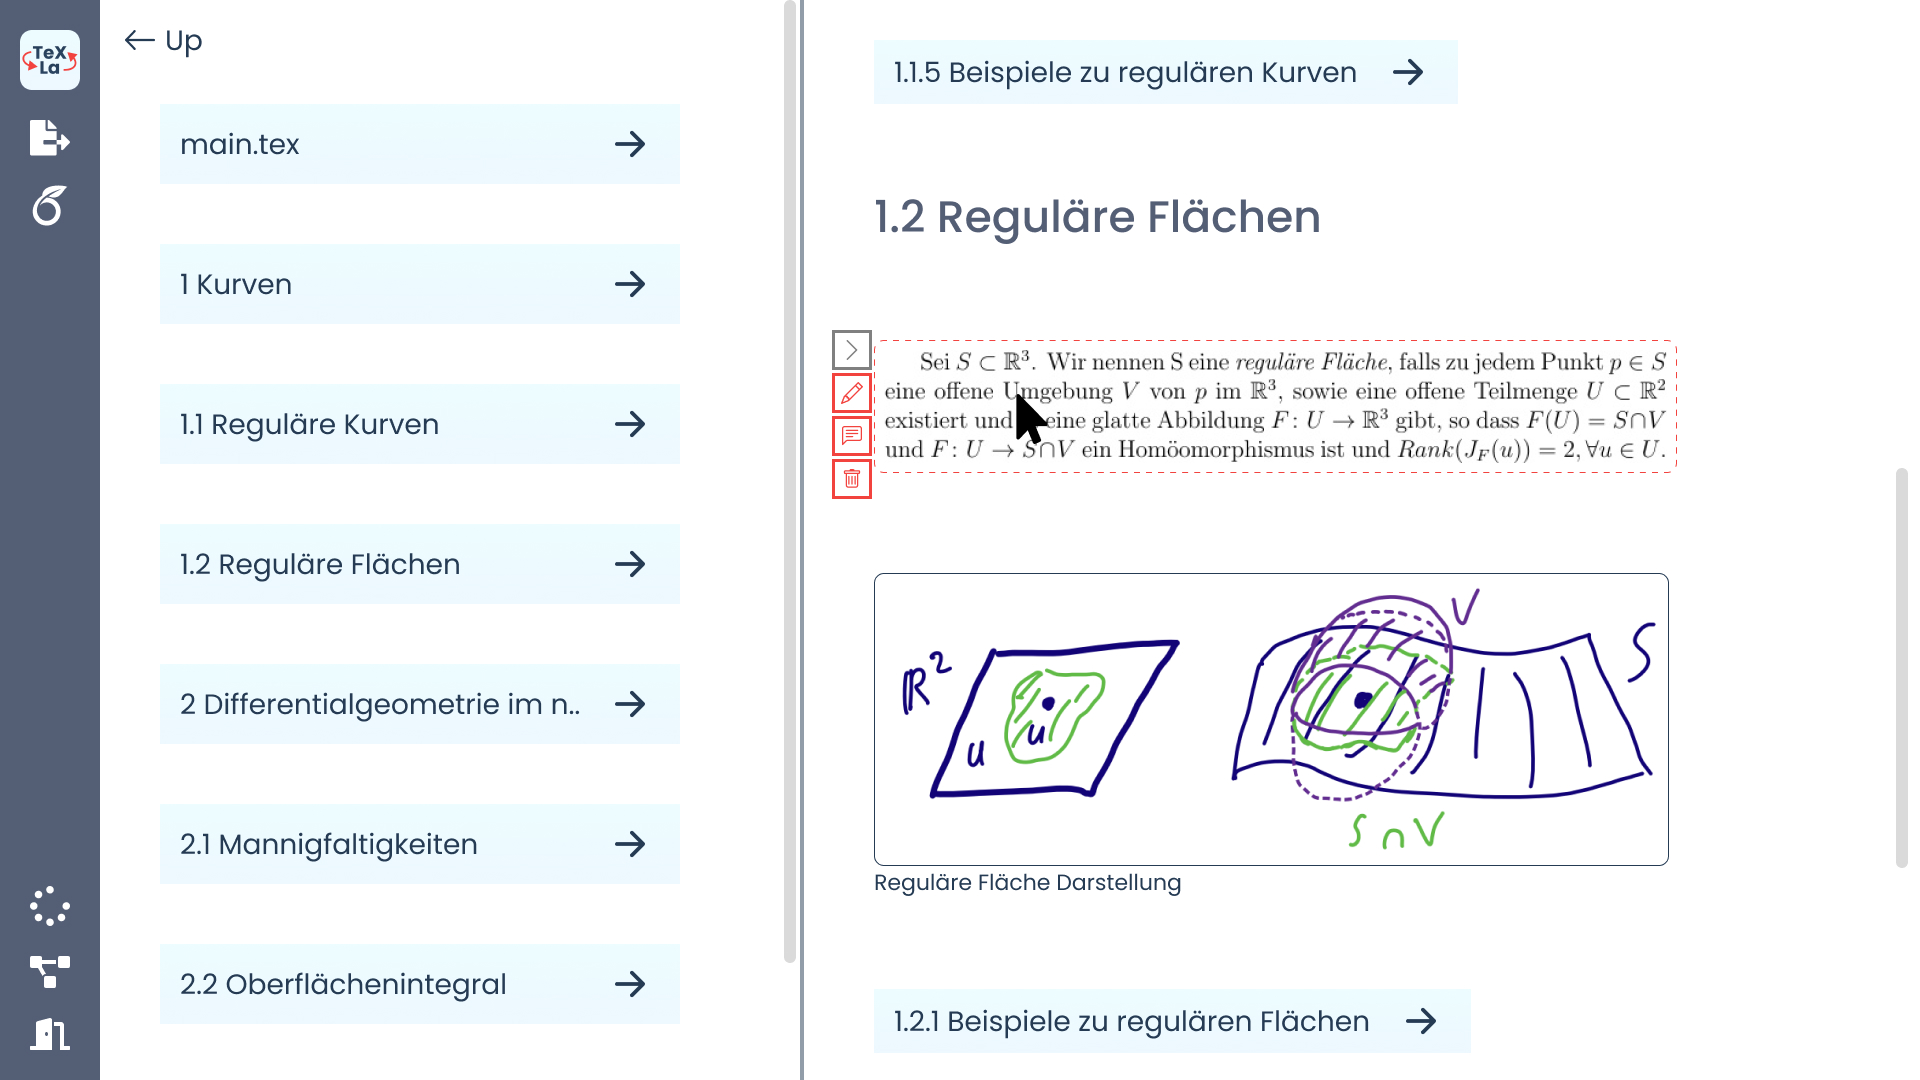
\includegraphics[width=\textwidth]{assets/img/Item_Selected_Hover}
  \captionof{figure}{Element fokussieren}
\end{minipage}

Ein Element in der Standardansicht kann in der rechten Spalte durch Hovern fokussiert werden.
Es erscheint eine Seitenleiste mit den Optionen \enquote{Expandable auswählen}, \enquote{Bearbeiten} und
\enquote{Löschen}.
Die erste Option ist nur bei Expandables aktiv und nutzbar.

\subsubsection{Löschen}

Diese Option löscht das fokussierte Element.

\subsubsection{Expandable auswählen}

\begin{minipage}{\linewidth}
  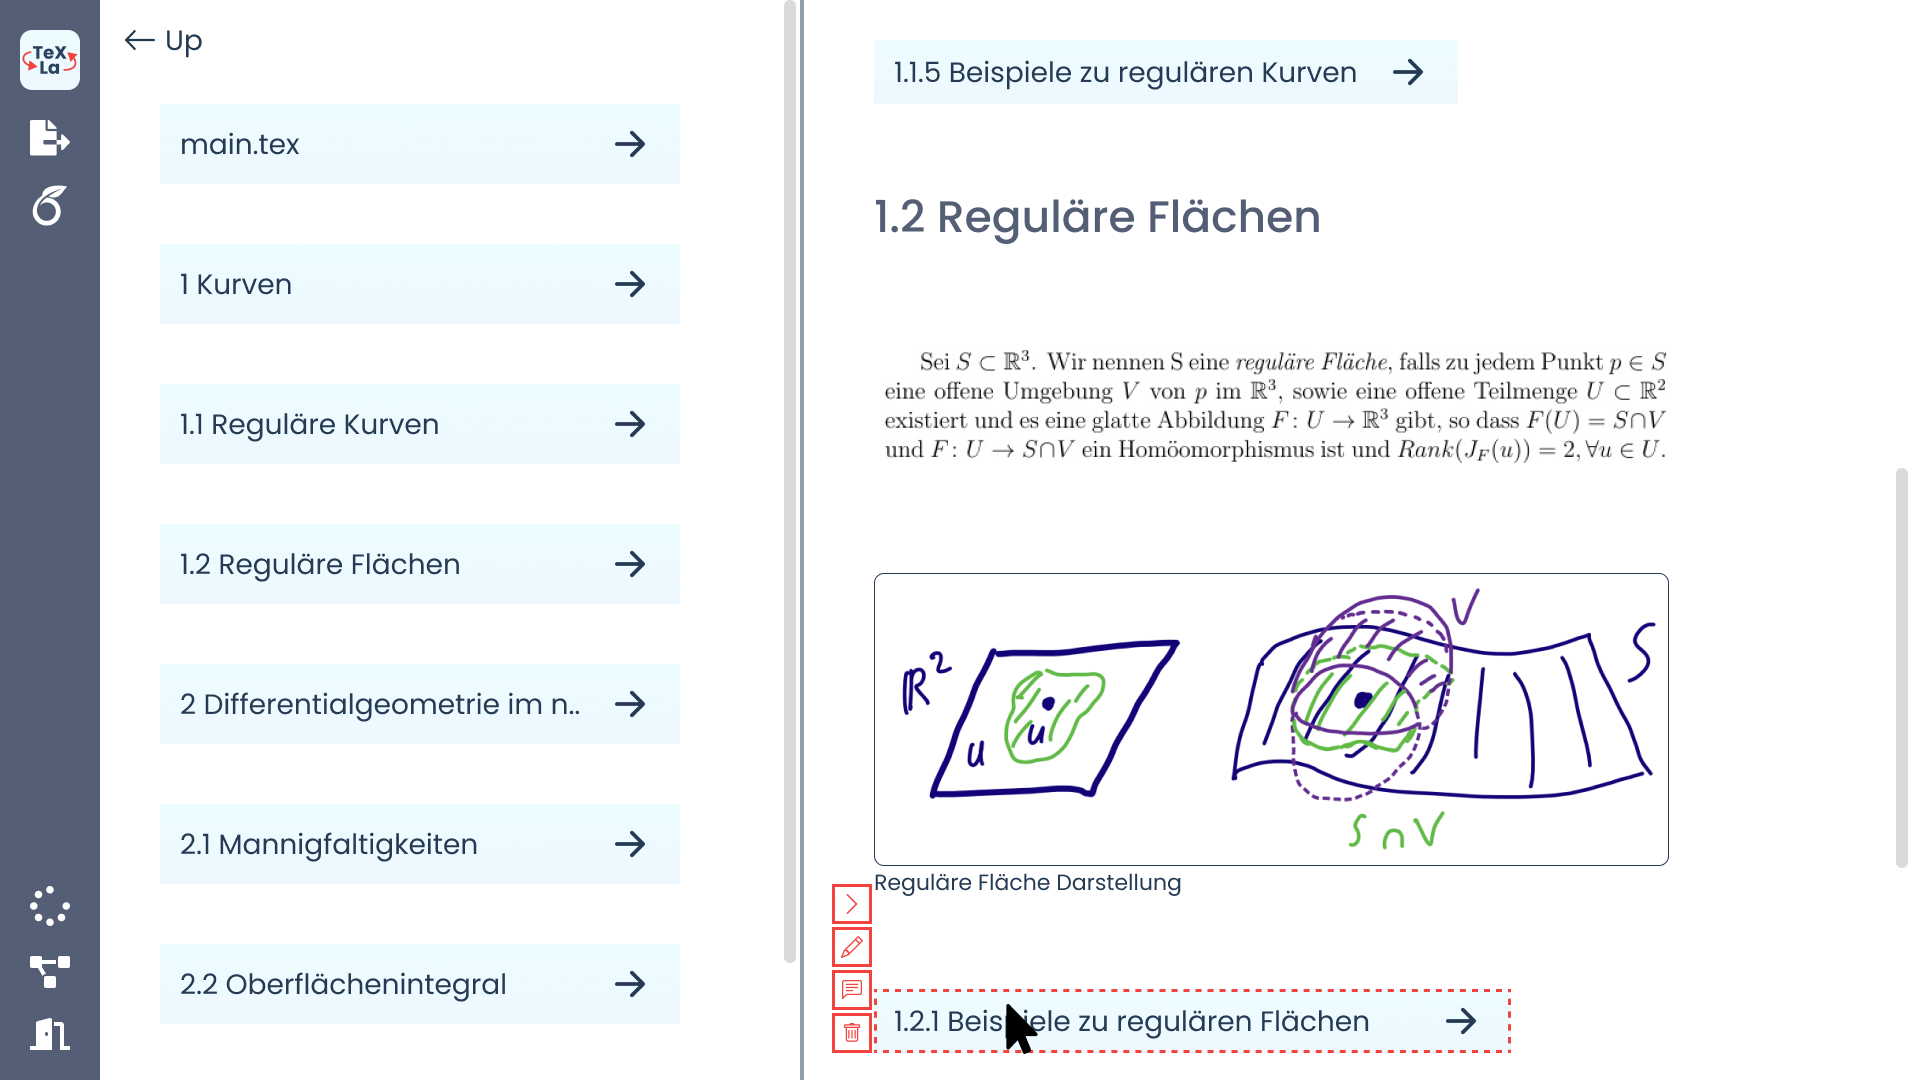
\includegraphics[width=\textwidth]{assets/img/Select_Expandable}
  \captionof{figure}{Expandable auswählen}
\end{minipage}

Durch Klicken der \enquote{Expandable auswählen}-Option bei fokussierten Expandables in der rechten Spalte wechseln
beide Spalten eine Ebene niedriger.
Durch einen Klick auf den Up-Button links oben im Navigationsbereich wechseln beide Spalten eine Ebene höher.

\subsection{Element hinzufügen}
\label{subsec:element-hinzufuegen}

\begin{minipage}{\linewidth}
  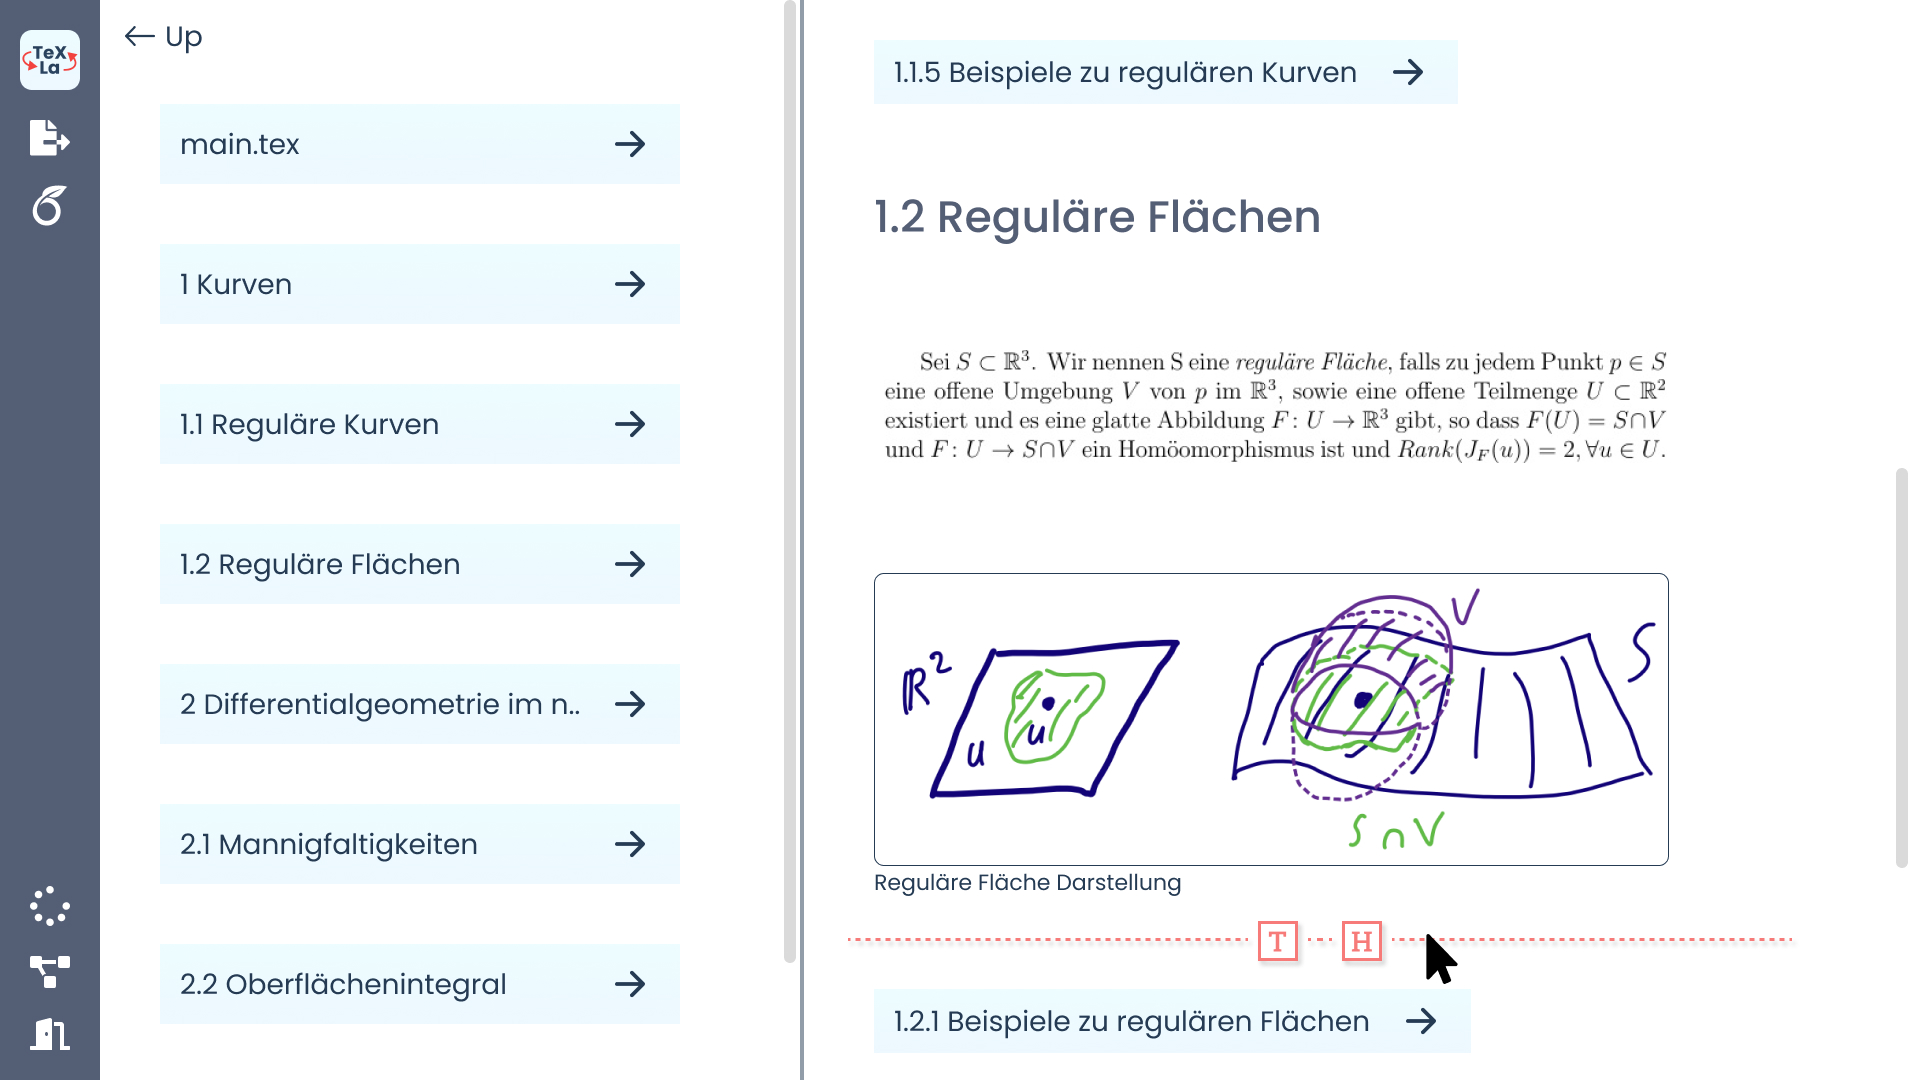
\includegraphics[width=\textwidth]{assets/img/Item_Add_Hover}
  \captionof{figure}{Element hinzufügen durch Hovern}
\end{minipage}

Der User kann durch Hovern zwischen Elementen andere Elemente hinzufügen.
Der Zwischenraum, welcher mit dem neuen Element gefüllt werden soll, wird fokussiert.

\clearpage

\subsubsection{Abschnitt hinzufügen}

Nachdem der \enquote{Abschnitt hinzufügen}-Button gedrückt wurde, erscheint ein Popup-Fenster.

\begin{center}
  \begin{minipage}{0.5\linewidth}
    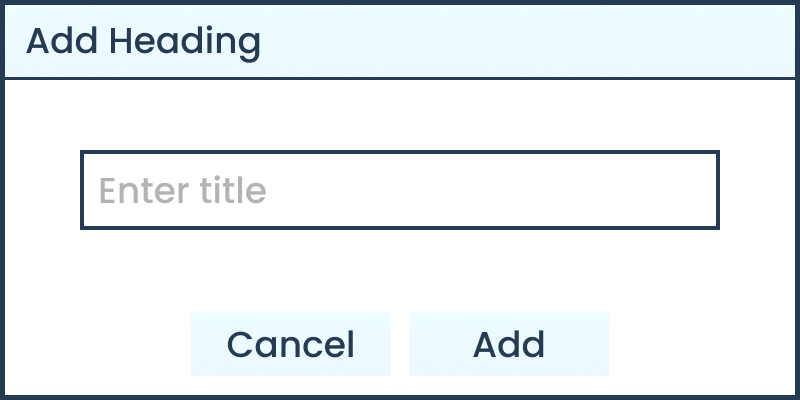
\includegraphics[width=\textwidth]{assets/img/Add_Heading_Box}
    \captionof{figure}{Abschnitt hinzufügen}
  \end{minipage}
\end{center}

Im \enquote{Abschnitt hinzufügen}-Fenster kann der User eine Überschrift für einen neuen Abschnitt eingeben und den
Vorgang bestätigen oder abbrechen.
